\documentclass[11pt]{article}
\usepackage[T1]{fontenc}
\usepackage{lmodern,microtype,amsmath,amssymb,amsthm,mathtools}
\usepackage[a4paper,margin=26mm]{geometry}
\usepackage{graphicx,booktabs,array,enumitem,fancyhdr,xcolor}
\usepackage[colorlinks=true,linkcolor=teal!65!black,citecolor=teal!65!black,urlcolor=teal!65!black]{hyperref}
\graphicspath{{figures/}}
\newtheorem{theorem}{Theorem}
\newtheorem{proposition}[theorem]{Proposition}
\newtheorem{corollary}[theorem]{Corollary}
\newtheorem{lemma}[theorem]{Lemma}
\theoremstyle{definition}\newtheorem{definition}[theorem]{Definition}
\newcommand{\R}{\mathbb R}
\newcommand{\diag}{\operatorname{diag}}
\newcommand{\tr}{\operatorname{tr}}
\newcommand{\rank}{\operatorname{rank}}
\newcommand{\cond}{\operatorname{cond}}
\newcommand{\opt}{\mathcal K}
\newcommand{\sgn}{\operatorname{sign}}
\DeclareMathOperator*{\argmax}{arg\,max}
\setlist{nosep,leftmargin=*}
\setlength{\parskip}{3pt}
\setlength{\parindent}{1.2em}
\pagestyle{fancy}\fancyhf{}\fancyhead[L]{\small Shivam Gupta}\fancyhead[R]{\small Residual-diagonal certificates}\fancyfoot[C]{\thepage}
\setlength{\headheight}{14pt}
\title{Diagonal Certificates for Nystr\"om Preconditioners:\\Exact Worst Cases and a Vector-Balancing Barrier}
\author{Shivam Gupta\\\small Independent Researcher, India\\\small\href{mailto:shivam1720406@gmail.com}{shivam1720406@gmail.com}}
\date{17 October 2026}
\begin{document}
\maketitle
\begin{abstract}
Partial Cholesky and column Nystr\"om methods maintain a positive-semidefinite residual diagonal at little additional cost. Can that information certify a substantially better preconditioned condition number than the familiar residual-trace bound? We characterize the strongest universal certificate consistent with an SPD preconditioner and a prescribed PSD residual diagonal. Its exact value is one plus a positive-semidefinite binary quadratic optimum, attained by a rank-one residual. For a rank-$k$ approximation with ridge regularization, Woodbury's identity converts this optimum into a $k$-dimensional vector-balancing problem. Classical floating-variable rounding then gives an explicit lower bound on every valid diagonal-only upper certificate, determined by the $k$ largest residual-weighted ridge leverage scores. The resulting barrier is sharp in the general low-rank class; exact evaluation remains NP-hard even for a one-column Nystr\"om transcript. On 360 kernel systems from three real datasets, the barrier retains median 98.71--99.36\% of the trace bound's excess above one, although actual median condition numbers are 29.7--46.1. At target condition number ten, all 107 actually qualifying systems remain impossible to accept universally from the recorded information. Exhaustive small cases, explicit adversarial completions, semidefinite brackets, and larger factor-based checks accompany the proofs. The result identifies when improved stopping decisions require additional residual information rather than more elaborate processing of the same diagonal.
\end{abstract}
\noindent\textbf{Keywords:} Nystr\"om approximation; preconditioned conjugate gradients; residual diagonals; vector balancing; semidefinite relaxation; kernel methods.\\
\textbf{Reproducibility:} \url{https://github.com/shi1720/residual-diagonal-certificates}.

\section{Introduction}
Low-rank preconditioning is effective when a relatively small approximation captures the costly spectral directions of a regularized kernel matrix. Constructing the approximation can nevertheless dominate a short solve. An adaptive implementation needs a stopping decision: has it gathered enough information to justify the desired spectral guarantee?

For a PSD matrix $A$, a partial Cholesky factor $F\in\R^{n\times k}$ gives
\begin{equation}\label{eq:model}
 A=FF^T+R,\qquad R\succeq0,\qquad P=FF^T+\mu I,\quad \mu>0.
\end{equation}
The factorization maintains $r=\diag(R)$ without evaluating every residual entry. A familiar sufficient bound is
\begin{equation}\label{eq:trace}
 \cond\bigl(P^{-1/2}(A+\mu I)P^{-1/2}\bigr)
 \le 1+\frac{\tr R}{\mu}=1+\frac{\sum_i r_i}{\mu}.
\end{equation}
A large right-hand side is often interpreted as a weak analysis. Sometimes it instead reflects an unavoidable limitation of the information being analyzed. A diagonal identifies the remaining coordinate energies, but leaves their alignment unresolved. The distinction matters when deciding whether to invest in a more expensive certificate, acquire residual matrix--vector products, or continue factorization.

This paper asks an information question: among \emph{all PSD residuals} having the observed diagonal, what is the largest possible preconditioned condition number? The answer defines the smallest upper certificate that can be valid uniformly over that uncertainty set. It is separate from the condition number of the actual residual and from the iteration count of a particular right-hand side.

Our main result is an exact characterization of this quantity. A rank-one residual is sufficient to attain the worst case, even though the uncertainty set contains matrices of every rank. The characterization reduces the problem to positive-semidefinite binary quadratic optimization. In the low-rank setting~\eqref{eq:model}, a complementary vector-balancing formulation yields a stronger and inexpensive information barrier. It depends on only the largest $k$ residual-weighted ridge leverage scores, rather than their full sum.

The contributions are:
\begin{enumerate}
\item An exact worst-case condition-number formula, including an admissible rank-one witness and a proof that the same uncertainty remains after observing a complete column Nystr\"om transcript.
\item A sharp top-rank leverage barrier obtained by applying classical floating-variable rounding to the low-rank inverse geometry. It quantifies the maximum possible improvement over the residual-trace certificate.
\item A rank-one Nystr\"om embedding of number partitioning, establishing NP-hardness of exact evaluation even at approximation rank one; and a practical bracketing protocol using analytic bounds, explicit signs, and a classical SDP relaxation.
\item Reproducible computational evidence from exhaustive small cases, 360 kernel systems, 54 SDP cases, 216 kernel/pivot sensitivity cases, and 36 larger factor-based cases. These experiments distinguish spectral information limits from observed solver behavior.
\end{enumerate}
The binary quadratic relaxation, Woodbury identity, and floating-variable method are established tools. Our contribution is their specialization to the information retained by a Nystr\"om preconditioning transcript, especially the resulting top-rank barrier and its operational interpretation. We do not propose a new low-rank approximation algorithm or claim a faster kernel solver.

\section{Related work and the contribution boundary}
\paragraph{Nystr\"om preconditioning.}
Frangella, Tropp, and Udell analyze randomized Nystr\"om PCG, effective-dimension rank requirements, and adaptive rank selection~\cite{ftu}. Their adaptive procedures use residual norm estimation through additional operator applications. D\'iaz et al. develop robust kernel ridge regression preconditioners, including RPCholesky and KRILL~\cite{diaz}. Abedsoltan et al. analyze how Nystr\"om approximation affects preconditioning in kernel machines~\cite{abed}. Those works establish the algorithmic setting and practical importance. We study the strongest \emph{deterministic, transcript-conditional} guarantee available before further residual observations. Our $P=FF^T+\mu I$ is the ridge-shifted approximation, not every spectrally rescaled Nystr\"om preconditioner.

\paragraph{Partial Cholesky and residual diagonals.}
Chen et al. explain the column Nystr\"om identity, residual-diagonal pivoting, trace stopping rules, and RPCholesky guarantees~\cite{chen}. Epperly, Tropp, and Webber accelerate that algorithm using rejection sampling~\cite{accelerated}. Epperly's recent analysis obtains stronger spectral-error and preconditioning guarantees with high probability~\cite{epperly2026}. These distributional statements exploit how the sketch was generated. They do not assert that every PSD completion of a realized transcript has equally good conditioning. Our universal-completion requirement is stronger and deliberately different: a low-probability but compatible completion is enough to rule out such a certificate. We do not challenge probabilistic rank guarantees.

\paragraph{Quadratic optimization and discrepancy.}
Rohn's work connects mixed matrix norms and the complexity of robust linear-algebra questions~\cite{rohn}. Nesterov's semidefinite relaxation gives the classical $\pi/2$ bound for PSD binary quadratic optimization~\cite{nesterov}. We use that relaxation as a computational bracket; it is not a new optimization method. The basic-feasible-solution or floating-variable approach in discrepancy theory leaves at most the constraint rank many coordinates fractional. Gupta et al. use this principle in a substantially different dynamic discrepancy setting~\cite{discrepancy}. Here it bounds a Euclidean balancing penalty after the Woodbury transformation. Both the rounding technique and conditional expectation are classical; the residual-weighted top-rank expression is the application-specific quantity.

\begin{table}[t]
\centering\small
\caption{Questions distinguished by the information used. A stronger information model can support a guarantee excluded by a weaker one.}
\begin{tabular}{>{\raggedright\arraybackslash}p{.28\linewidth}>{\raggedright\arraybackslash}p{.32\linewidth}>{\raggedright\arraybackslash}p{.31\linewidth}}
\toprule
Setting & Available information & Principal guarantee\\\midrule
Randomized Nystr\"om PCG~\cite{ftu} & Sketch and further residual products & Adaptive spectral/solve guarantees\\
RPCholesky analysis~\cite{chen,epperly2026} & Matrix class and randomized sampling process & Error or conditioning with stated probability\\
PSD quadratic relaxation~\cite{nesterov} & A supplied PSD quadratic objective & Approximation of a sign optimum\\
Present information audit & Realized factor, ridge, and residual diagonal & Exact universal-completion optimum and a lower barrier on any valid upper certificate\\\bottomrule
\end{tabular}
\end{table}

\section{The strongest universal residual-diagonal certificate}
Let $P\in\R^{n\times n}$ be SPD, let $r\in\R_+^n$, and assume $n\ge2$. Define
\begin{equation}
 \mathcal U(r)=\{R\succeq0:\diag(R)=r\},\qquad
 \opt(P,r)=\max_{R\in\mathcal U(r)}
 \cond\bigl(I+P^{-1/2}RP^{-1/2}\bigr).
\end{equation}
The maximum exists: PSD matrices with prescribed diagonal form a compact set, and the matrices inside the condition number are uniformly positive definite. A universal diagonal certificate is a function $C(P,r)$ satisfying $C(P,r)\ge\opt(P,r)$. Thus $\opt$ is a \emph{lower bound on any valid upper certificate}, not a lower bound on the actual condition number.

Write $D=\diag(\sqrt{r_1},\ldots,\sqrt{r_n})$ and $B=DP^{-1}D$. Coordinates with $r_i=0$ may be removed from the sign problem: PSD Cauchy--Schwarz implies that their residual rows and columns vanish.

\begin{theorem}[Exact worst case]\label{thm:exact}
For $n\ge2$,
\begin{equation}\label{eq:exact}
 \opt(P,r)=1+f(P,r),\qquad
 f(P,r)=\max_{s\in\{-1,1\}^n}s^TBs.
\end{equation}
A maximizing sign vector $s_\star$ supplies an attaining residual
$R_\star=(Ds_\star)(Ds_\star)^T$. Equivalently,
$f(P,r)=\|P^{-1/2}D\|_{\infty\to2}^2$.
\end{theorem}
\begin{proof}
Represent $R\in\mathcal U(r)$ as a Gram matrix, $R_{ij}=u_i^Tu_j$, with $\|u_i\|_2=\sqrt{r_i}$. For every unit $z$, put $a=P^{-1/2}z$. Then
\begin{align}
 z^TP^{-1/2}RP^{-1/2}z
 &=\Big\|\sum_i a_i u_i\Big\|_2^2
 \le\Big(\sum_i |a_i|\sqrt{r_i}\Big)^2\\
 &=\max_{s\in\{-1,1\}^n}(z^TP^{-1/2}Ds)^2.
\end{align}
Maximizing over $z$ and exchanging the finite sign maximum gives an upper bound $f(P,r)$ on the largest eigenvalue of the relative residual. Its smallest eigenvalue is nonnegative, so the condition number is at most $1+f(P,r)$.

For $v=Ds_\star$, the matrix $P^{-1/2}vv^TP^{-1/2}$ has one potentially nonzero eigenvalue $v^TP^{-1}v=f(P,r)$ and at least one zero eigenvalue. The preconditioned system therefore has condition number exactly $1+f(P,r)$. This also covers $r=0$. Finally, a convex quadratic on the cube $[-1,1]^n$ attains a maximum at a vertex, yielding the mixed-norm identity.
\end{proof}
The restriction $n\ge2$ is necessary: every positive scalar has condition number one. No assumption that $P$ and $R$ commute is used.

\subsection{Why a column Nystr\"om transcript does not remove the adversary}
Let $S$ be a landmark set with $A_{SS}\succ0$, and choose $F=A_{:S}A_{SS}^{-1/2}$. The column Nystr\"om approximation is $FF^T$, and its residual satisfies $R_{:S}=0$. Consequently, $r_i=0$ for $i\in S$.

Conversely, fix a factor consistent with these observed columns. Every $R\in\mathcal U(r)$ has zero rows and columns on $S$. The completion $A'=FF^T+R$ is PSD, agrees with every observed column and diagonal entry, and yields the same Nystr\"om factor. Thus Theorem~\ref{thm:exact} remains exact after conditioning on this complete transcript. For partial Cholesky, the intermediate residual diagonals are also determined by $F$ and the original diagonal. Hence they do not exclude these completions.

Additional constraints can shrink the uncertainty set. A supplied Gaussian-kernel formula and all input coordinates, an independent residual probe, or a general non-coordinate sketch may provide information beyond this transcript. The theorem does not claim that the constructed adversary is an RBF kernel on the original dataset.

\begin{figure}[t]
\centering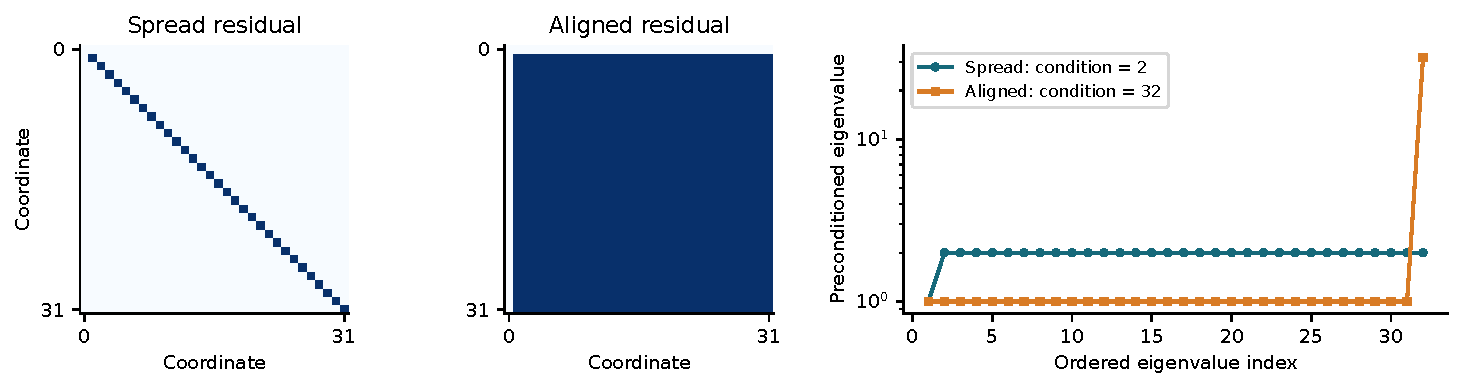
\includegraphics[width=\linewidth]{same_diagonal.pdf}
\caption{An exact ambiguity example. Take $n=32$, $F=3e_1$, $\mu=1$, and $r=(0,1,\ldots,1)$. Both residuals are PSD, have the same diagonal, and preserve the first observed column. The spread residual gives condition number two; the aligned rank-one residual gives condition number 32. These are analytic spectra, not measured solver times.}\label{fig:example}
\end{figure}

\section{A low-rank vector-balancing barrier}
Return to $P=FF^T+\mu I$, where $F$ has $k\ge1$ columns. Set
\begin{equation}\label{eq:V}
 G=F^TF+\mu I,\qquad V=G^{-1/2}F^TD,
 \qquad h_i=\bigl(FG^{-1}F^T\bigr)_{ii},\qquad a_i=r_i h_i.
\end{equation}
Only the Gram matrix $V^TV$ matters; a Cholesky-based square-root factor gives the same column norms and balancing objective. Woodbury's identity gives
\begin{equation}\label{eq:balance}
 B=\mu^{-1}(D^2-V^TV),\qquad
 f(P,r)=\frac{\sum_i r_i-\min_{s\in\{-1,1\}^n}\|Vs\|_2^2}{\mu}.
\end{equation}
The vectors being balanced are the columns of $V$, with squared norms $a_i$. Alignment of the residual can almost saturate the trace certificate when those vectors admit a good signing.

Let $a_{(1)}\ge\cdots\ge a_{(n)}$ be the ordered $a_i$, let $q=\min(k,n)$, and write $T=\sum_i r_i/\mu$. Define
\begin{equation}\label{eq:barriers}
 L_0=T-\frac{\sum_i a_i}{\mu},\qquad
 L_k=T-\frac{\sum_{j=1}^{q}a_{(j)}}{\mu}.
\end{equation}

\begin{theorem}[Top-rank information barrier]\label{thm:barrier}
Every universal residual-diagonal certificate obeys
\begin{equation}\label{eq:chain}
 C(P,r)\ \ge\ \opt(P,r)=1+f(P,r)
 \ \ge\ 1+L_k\ \ge\ 1+L_0,
 \qquad f(P,r)\le T.
\end{equation}
The term $L_k$ can use $\rank(V)$ in place of $k$. There is a constructive signing with $\|Vs\|_2^2\le\sum_{j=1}^{q}a_{(j)}$, obtainable by floating-variable rounding and conditional expectation. The top-rank penalty is attained on some low-rank instances, so it cannot be uniformly decreased over the whole stated class.
\end{theorem}
\begin{proof}
Consider the nonempty bounded polytope
$\mathcal P=\{x\in[-1,1]^n:Vx=0\}$.
At a vertex $x$, at most $\rank(V)$ coordinates are strictly between $-1$ and $1$. Otherwise the columns corresponding to fractional coordinates have a nonzero linear dependence, which permits a small feasible displacement in both directions and contradicts extremality.

Keep integral coordinates fixed. Round each fractional coordinate independently to a sign $s_i$ with mean $x_i$. Because $Vx=0$, independence and zero-mean rounding errors imply
\begin{equation}
 \mathbb E\|Vs\|_2^2
 =\sum_{i:\,|x_i|<1}(1-x_i^2)\|V_{:i}\|_2^2
 \le\sum_{j=1}^{q}a_{(j)}.
\end{equation}
Sequential conditional expectation selects a deterministic outcome no larger than this expectation. Substitution into~\eqref{eq:balance} proves the stronger lower bound. The weaker one also follows directly from a uniformly random sign vector, since $\mathbb E\|Vs\|_2^2=\sum_i a_i$, or from $f\ge\tr B=L_0$. Finally $B\preceq D^2/\mu$ gives $f\le T$.

For sharpness, choose $F$ nonzero on only $k<n$ rows, with these rows mutually orthogonal and all other rows zero. Then the nonzero columns of $V$ are mutually orthogonal. Every signing has the same penalty, equal to the sum of those $k$ squared column norms. Hence $f=L_k$. An analogous column-transcript construction appends $k$ landmark rows to this factor, sets their residual diagonals to zero, and retains one orthogonal active residual coordinate per column.
\end{proof}

\subsection{How much can a diagonal-only analysis improve?}
When $r\ne0$, define the top-rank overlap fraction
\begin{equation}
 \theta_k=\frac{\sum_{j=1}^{q}a_{(j)}}{\sum_i r_i}.
\end{equation}
The best possible certificate's excess above one lies in
\begin{equation}\label{eq:theta}
 T(1-\theta_k)\le \opt(P,r)-1\le T.
\end{equation}
Thus no universal diagonal-only method can improve the trace certificate's excess by more than the fraction $\theta_k$. The statement concerns the best possible certificate, regardless of computation time.

A coarser interpretation uses $n_{\rm eff}=\sum_i r_i/\max_i r_i$ and $h_{\max}=\max_i h_i$:
\begin{equation}
 \theta_k\le \frac{k h_{\max}}{n_{\rm eff}},\qquad
 \frac{\sum_i a_i}{\sum_i r_i}
 \le\frac{\tr(FG^{-1}F^T)}{n_{\rm eff}}\le\frac{k}{n_{\rm eff}}.
\end{equation}
The top-rank expression improves substantially on the full overlap sum when residual-weighted leverage is diffuse. Computing the $h_i$ costs $O(nk^2+k^3)$ arithmetic with $O(nk+k^2)$ storage; selecting the largest $k$ values needs no dense $n\times n$ inverse. This is an audit of a fixed transcript. Increasing the approximation rank changes $r$ and $F$, so these inequalities are not a lower bound on the rank required by every adaptive approximation algorithm.

\subsection{Exact evaluation is hard even at rank one}
\begin{proposition}\label{prop:hard}
Exact evaluation of $\opt(P,r)$ is NP-hard for rational inputs even when $\mu=1$, $F$ has one column, and the information is a valid one-column Nystr\"om transcript.
\end{proposition}
\begin{proof}
Given positive integers $u_1,\ldots,u_m$ from \textsc{Partition}, take
$F=(1,u_1,\ldots,u_m)^T$ and $r=(0,1,\ldots,1)^T$.
The first coordinate is the landmark. Every compatible residual has a zero first row, so the observed first column and the one-column Nystr\"om factor are preserved. Equation~\eqref{eq:balance} becomes
\begin{equation}
 f(P,r)=m-\frac{\min_{s\in\{-1,1\}^m}(\sum_i u_i s_i)^2}{2+\sum_i u_i^2}.
\end{equation}
Consequently, $\opt(P,r)=m+1$ if and only if the integers admit a perfect partition. The construction has polynomial bit length. This establishes NP-hardness through the classical \textsc{Partition} problem~\cite{karp}; it is not a strong-NP-hardness claim.
\end{proof}
This result explains why a simple closed formula need not exist even though the attaining residual has rank one. The hard choice is its coordinatewise orientation.

\section{A practical bracketing and information-acquisition protocol}
For a desired condition-number ceiling $\tau>1$, compute an upper bound $U\ge f(P,r)$ and a lower bound $L\le f(P,r)$. Suitable lower bounds include $L_k$ and any sign objective. The protocol has three outcomes:
\begin{enumerate}
\item If $1+U\le\tau$, the transcript supports universal acceptance.
\item If $1+L>\tau$, universal acceptance is impossible from this transcript. Acquire additional residual information or change the approximation.
\item Otherwise, the current bracket is unresolved; tighter optimization may decide it.
\end{enumerate}
The second outcome does not reject the actual preconditioner. It rejects a proposed \emph{universal guarantee} based on the available information. This distinction is central to avoiding unnecessary factorization.

\paragraph{Cheap bounds and explicit witnesses.}
Equation~\eqref{eq:trace} provides $U=T$ in the low-rank model. For general $P$, $\sum_{ij}|B_{ij}|$ and $m\lambda_{\max}(B)$ are also upper bounds, where $m$ is the number of active residual coordinates. Signs provide directly checkable PSD residuals $Ds s^TD$ and lower bounds $s^TBs$. We implement seeded coordinate ascent for these signs and the constructive floating-variable method. Neither is claimed to solve the sign problem globally.

\paragraph{Classical semidefinite brackets.}
A stronger optional upper bound is
\begin{equation}\label{eq:sdp}
 S(B)=\max_{X\succeq0,\,\diag X=\mathbf1}\langle B,X\rangle
 =\min_{y:\,\diag(y)-B\succeq0}\mathbf1^Ty.
\end{equation}
Strict feasibility yields strong duality. The classical PSD Grothendieck bound gives
\begin{equation}
 f(P,r)\le S(B)\le\frac{\pi}{2}f(P,r).
\end{equation}
Appendix~\ref{app:sdp} recalls the argument. In the low-rank model, $y=r/\mu$ is already dual feasible because $\diag(r/\mu)-B=V^TV/\mu\succeq0$. The balancing barrier therefore quantifies how little room can remain for an expensive SDP improvement over this explicit feasible dual.

\paragraph{Numerical status.}
The mathematical certificates above are exact-arithmetic statements. Our implementation uses double precision. It symmetrizes computed matrices, repairs SDP dual vectors by a positive eigenvalue-based shift, retains minimum dual eigenvalues, and checks witnesses against generalized eigenvalues. These are numerical validation steps, not outward-rounded interval certificates. A deployment requiring formally rigorous floating-point guarantees needs verified inverse products and PSD checks. A numerically feasible primal SDP objective is not used as an upper certificate.

\section{Computational study}
\subsection{Design and reproducibility}
The complete implementation, retained JSON records, tests, and figure scripts are available in the artifact. Results below are descriptive evaluations on fixed matrices, not population-level performance estimates.

\paragraph{Small-instance checks.}
We enumerate all sign vectors up to a global sign for 132 random SPD-preconditioner instances: twelve instances for each $n=2,\ldots,12$. For every instance, the attaining rank-one construction is checked using an independent generalized symmetric eigensolver. Three further PSD completions with the same diagonal are tested, giving 396 completion comparisons. Separate checks cover the Woodbury trace identity, diagonal preconditioners, and an integer Max-Cut identity. Another 150 instances check the balancing construction for $n\in\{4,8,12,32,100\}$ and $k\in\{1,2,3\}$. An exact partition example and an orthogonal-column tightness example are retained as regression cases.

\paragraph{Kernel systems.}
We use the feature matrices from scikit-learn 1.5.2's Digits, Wisconsin Diagnostic Breast Cancer, and Diabetes datasets~\cite{sklearn,street,efron}. Labels are not used. For each sampled subset, features are centered and divided by their empirical standard deviations; constant features are set to zero. The RBF kernel is
$K_{ij}=\exp(-\|x_i-x_j\|_2^2/b)$, where $b$ is the median off-diagonal squared distance.

We use $n\in\{128,256,512\}$ when the source dataset is large enough, five subset/pivot seeds, nested RPCholesky ranks $k\in\{8,16,32\}$, and $\mu\in\{0.01,0.1,1\}$. This gives 135 Digits, 135 Breast Cancer, and 90 Diabetes systems, for 360 total. The larger size is unavailable for the 442-row Diabetes dataset; it is not silently replaced. Kernel hashes are retained. RPCholesky is a direct implementation of residual-diagonal sampling~\cite{chen}, not the accelerated algorithm. Pivot residual coordinates are set to their theoretical zero values; negative roundoff-level diagonal remainders are clipped to zero.

For each system, dense generalized eigenvalues give the actual condition number. An explicit rank-one adversarial completion shares $F$, the diagonal, and every pivot column. SciPy PCG solves the actual and adversarial systems with the same Gaussian right-hand side, zero start, and relative residual tolerance $10^{-9}$. Right-hand sides vary across parameter settings; the reported iteration counts describe these solves and are not a controlled right-hand-side comparison across ranks.

\paragraph{Additional studies.}
A separate 54-case SDP study uses $n=64$, three datasets, three seeds, ranks $4,8,16$, and $\mu=0.1,1$. A 36-case factor-based study uses Digits subsets of sizes 1,024 and 1,797, three seeds, ranks $16,64,128$, and $\mu=0.1,1$. It evaluates the barrier and a constructed signing; it does not compute full condition numbers or claim a large-scale solve speedup. A 216-case sensitivity study crosses three datasets, three seeds, RBF/Mat\'ern-$3/2$/linear kernels, greedy/random pivoting, ranks $8,32$, and $\mu=0.1,1$, at $n=256$.

\subsection{Results}
\begin{table}[t]
\centering\small
\caption{Main kernel study. All numeric columns are medians across the listed cases. The barrier ratio compares \emph{excesses above one}; it is not a condition-number ratio. Different dataset sizes give unequal case counts.}\label{tab:main}
\begin{tabular}{lrrrrr}
\toprule
Dataset & Cases & Actual $\kappa$ & Trace upper & $L_k/T$ & PCG iters.\\\midrule
Digits & 135 & 46.1 & 1132.5 & 99.36\% & 48 \\
Breast cancer & 135 & 38.4 & 763.2 & 99.03\% & 46 \\
Diabetes & 90 & 29.7 & 477.2 & 98.71\% & 39 \\

\bottomrule
\end{tabular}
\end{table}

\paragraph{Verification.}
All small-instance checks pass. The largest relative discrepancy between $1+f$ and the attaining witness's generalized-eigenvalue condition number is $5.11\times10^{-15}$. All 150 balancing checks satisfy the top-rank penalty bound within $10^{-7}$ absolute tolerance; the largest LP equality residual is $6.00\times10^{-16}$. These finite checks corroborate the implementation; the universal claims follow from the proofs.

\paragraph{The trace certificate is nearly optimal for the recorded information.}
Table~\ref{tab:main} and Figure~\ref{fig:barrier} show that the top-rank barrier retains median 99.36\%, 99.03\%, and 98.71\% of $T$ for Digits, Breast Cancer, and Diabetes. The full relative-trace floor $L_0$ retains only 96.15\%, 95.49\%, and 94.20\% at the median. The top-rank argument therefore narrows the information-theoretic improvement budget substantially. Across individual main-study cases, $L_k/T$ ranges from 87.74\% to 99.96\%. The statement is conditional on these matrices and parameters; it is not a claim that residual-weighted leverage is always diffuse.

\begin{figure}[t]
\centering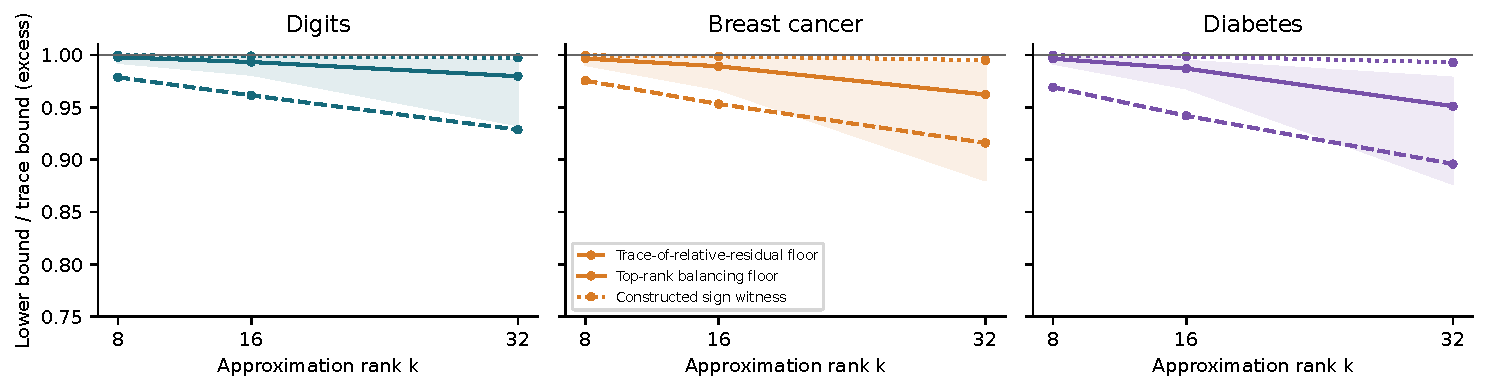
\includegraphics[width=\linewidth]{barrier.pdf}
\caption{Lower bounds on the best possible universal certificate, normalized by the residual-trace excess $T$. Lines show medians over sizes, seeds, and ridge values; shading shows the minimum--maximum range for the top-rank barrier. The dotted line uses the floating-variable witness. These are descriptive ranges, not confidence intervals.}\label{fig:barrier}
\end{figure}

\paragraph{The actual spectrum can be much better.}
Actual median condition numbers range from 29.7 to 46.1, while median trace certificates range from 477.2 to 1,132.5 (Figure~\ref{fig:gap}). The gap is not removed by optimizing over all compatible diagonal certificates: the lower barrier remains close to the trace bound. At target ten, all 107 actual systems meeting the target still have $1+L_k>10$. Table~\ref{tab:decisions} gives further thresholds. Thus a policy that insists on a universal transcript certificate would fail to recognize many actual spectral successes.

\begin{table}[t]
\centering\small
\caption{Threshold decisions among the 360 main-study systems. ``Blocked'' counts actual spectral successes whose transcript cannot support universal acceptance by Theorem~\ref{thm:barrier}. It does not count failed solves. Trace acceptance is always sufficient in exact arithmetic.}\label{tab:decisions}
\begin{tabular}{rrrr}
\toprule
Target $\tau$ & Actual $\kappa\le\tau$ & Of these, blocked & Trace accepts\\\midrule
10 & 107 & 107 & 0 \\
100 & 237 & 166 & 71 \\
1000 & 347 & 156 & 191 \\

\bottomrule
\end{tabular}
\end{table}

\begin{figure}[t]
\centering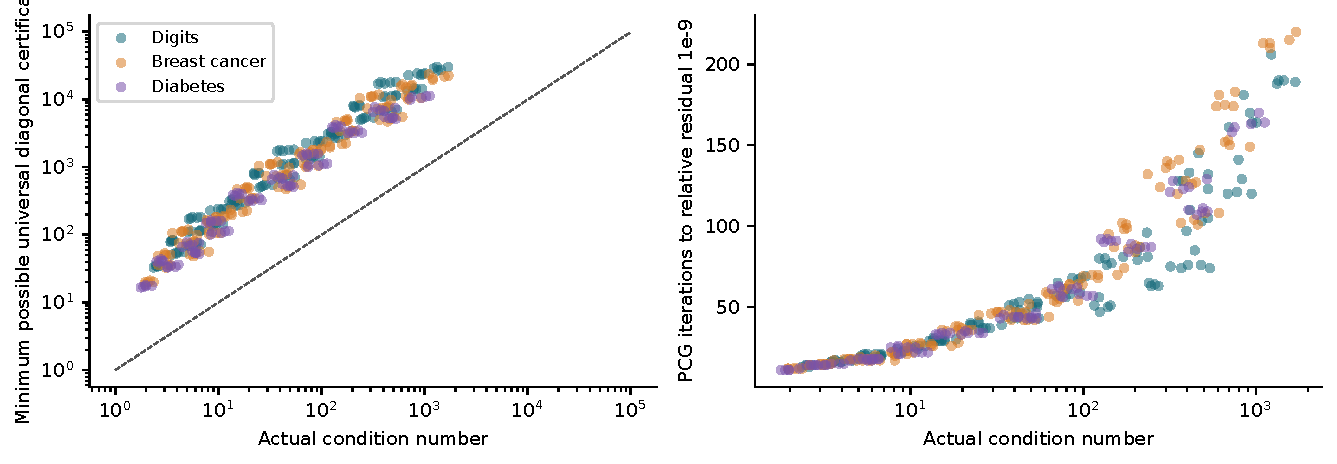
\includegraphics[width=\linewidth]{information_gap.pdf}
\caption{Actual systems and the transcript information limit. Left: actual condition number versus $1+L_k$; the dashed line marks equality. Right: measured PCG iterations for actual systems. Each point is one main-study case. The spectral information limit is not a solver-iteration lower bound.}\label{fig:gap}
\end{figure}

\paragraph{An expensive SDP usually has little room to improve.}
In the 54 smaller systems, the minimum of the repaired SDP dual and the trace certificate improves on $T$ by at most 0.00480\%; the median improvement is zero. The upper bracket is within 0.00087--0.6211\% of a constructed sign lower bound, with median relative gap 0.0482\% (Figure~\ref{fig:sdp}). Tiny raw repaired-dual excesses above the explicit trace dual are retained in the data rather than treated as improvements. These examples support using a cheap information barrier before invoking an SDP. They do not establish that the SDP is always tight or always unnecessary.

\paragraph{Larger factors and kernel sensitivity.}
In the 36 larger Digits cases, $L_k/T$ ranges from 96.68\% to 99.98\%, with median 99.48\%. The floating-variable implementation takes median 48.8\,ms per case in this recorded run, ranging from 6.3 to 284.6\,ms after factor construction. Timings are single-run, host-dependent measurements, not comparative speedups.

The sensitivity study retains 216 records. Twenty-four linear-kernel cases have residual-trace excess below $10^{-8}$ after the requested rank budget; they are excluded from ratios that would divide by an essentially zero trace. Among the remaining 192 cases, median $L_k/T$ is 99.20\%/99.32\% for RBF random/greedy pivoting, 99.35\%/99.39\% for Mat\'ern-$3/2$, and 98.15\%/99.05\% for linear kernels. Thus the observed barrier is not specific to the random pivot rule or the RBF family, although this remains a small benchmark collection.

\begin{figure}[t]
\centering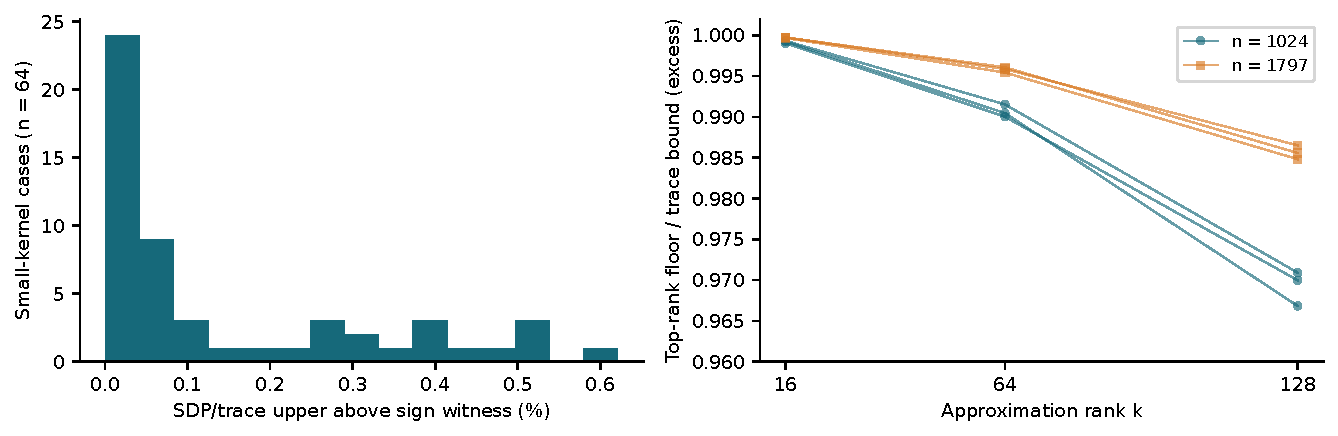
\includegraphics[width=\linewidth]{sdp_scaling.pdf}
\caption{Left: numerical upper/lower bracket gaps for 54 small-kernel cases, using the smaller of the trace and repaired SDP upper bounds. Right: the top-rank barrier for larger Digits matrices at $\mu=0.1$; each line is one seed. The complete larger study also includes $\mu=1$.}\label{fig:sdp}
\end{figure}

\paragraph{Conditioning and iterations must remain distinct.}
Every main-study solve reaches the required tolerance; the largest independently recomputed actual-system relative residual is below $9.99\times10^{-10}$. Actual median PCG iteration counts are 39--48. In contrast, every rank-one adversarial completion takes two PCG iterations in the experiment, despite potentially large condition numbers. In exact arithmetic such a matrix has only two distinct preconditioned eigenvalues. This is an instructive limitation: our extremizer witnesses a worst \emph{condition number}, not a worst CG trajectory. A service whose objective is iteration count rather than a spectral guarantee needs a different uncertainty objective.

\section{Implications, limitations, and next questions}
The result gives a concrete decision aid for kernel and Gaussian-process solver infrastructure. If $1+L_k$ already exceeds a required universal condition-number ceiling, more accurate optimization of the same transcript cannot meet that ceiling. A system can instead acquire a residual spectral estimate, use operator products as in adaptive Nystr\"om methods, or continue collecting columns. This can avoid spending effort on an impossible diagonal-only proof. It does not by itself establish an end-to-end runtime saving or a commercial return.

The uncertainty model is deliberately explicit. It uses PSD structure and the column transcript, not a probability distribution over unobserved residuals. It does not enforce a particular kernel function on known inputs. Distributional guarantees, additional entries, non-coordinate sketch constraints, and residual products can all exclude our adversarial completions. The theory does not apply unchanged to indefinite learned approximations, unverified one-sided residuals, or general spectrally rescaled preconditioners. If $R\succeq0$ is merely assumed by a model rather than established by construction, the certificate does not verify that assumption.

The exact optimum is computationally hard, but our main barrier is inexpensive and needs only the factor and residual diagonal. Its usefulness depends on leverage overlap. Concentrated residuals or leverage can leave a larger improvement budget. Our top-rank bound is sharp over the stated general class, yet it need not be tight for each transcript. The SDP bracket is an established relaxation, and the supplied floating-point implementation is not a formally verified numerical certificate engine.

The experiments emphasize interpretability and independent dense spectrum checks. They use small standard datasets and moderate matrix sizes; no GPU, distributed, or million-row performance claim is supported. Single-run timings lack uncertainty estimates and should not guide production procurement. The larger factor study extends the size of the information audit without replacing a full systems benchmark.

Two precise directions follow. First, characterize the strongest certificate after observing a small residual block or a few operator products: additional constraints can rule out rank-one completions, and the exact condition-number objective then becomes different. Second, formulate transcript uncertainty for a CG convergence functional that accounts for spectral clustering and right-hand-side alignment. The two-iteration adversarial example shows why a condition-number objective alone cannot answer that question.

\section{Conclusion}
A residual diagonal is inexpensive to maintain but can preserve substantial ambiguity in preconditioned conditioning. Its strongest universal certificate is exactly a PSD sign optimum. For ridge-shifted low-rank approximations, a vector-balancing formulation yields a top-rank leverage barrier that is close to the conventional trace bound on the tested kernel systems. The practical consequence is an information-acquisition criterion: before seeking a stronger certificate from a fixed transcript, check whether that transcript can support the requested guarantee at all.

\appendix
\section{The classical PSD semidefinite bracket}\label{app:sdp}
For completeness, let $X$ solve the primal SDP in~\eqref{eq:sdp}, and draw a centered Gaussian vector $g$ with covariance $X$. The signs $s_i=\sgn(g_i)$ satisfy
\begin{equation}
 \mathbb E[ss^T]=\frac2\pi\arcsin[X],
\end{equation}
where arcsine acts entrywise. The power-series coefficients of $\arcsin(t)-t$ are nonnegative. By the Schur product theorem, $\arcsin[X]-X\succeq0$. Since $B\succeq0$,
\begin{equation}
 \mathbb E[s^TBs]=\frac2\pi\langle B,\arcsin[X]\rangle
 \ge\frac2\pi\langle B,X\rangle=\frac2\pi S(B).
\end{equation}
Some sign therefore has value at least $2S(B)/\pi$, proving the stated bracket~\cite{nesterov}. A finite number of random rounds does not guarantee that it finds this expectation-achieving sign; the code reports the objective of the actual retained sign.

The implementation solves the primal with CVXPY 1.6.5 and Clarabel 0.11.1, rescales the objective by $\max(\|B\|_2,10^{-30})$, and extracts a dual vector. Given numerical $y$, it forms $M=\diag(y)-B$ and adds
\begin{equation}
 \delta=\max(0,-\lambda_{\min}(M))+10^{-10}\max(1,\|B\|_F)
\end{equation}
to every coordinate. The minimum eigenvalue of the repaired slack is recorded. This makes the reported dual numerically PSD in the retained cases; it is not an interval-arithmetic proof for the exact input. The analytical $T$ bound remains independently available for every low-rank case.

\section{Constructive rounding and implementation details}
The factor-based routine forms a Cholesky factor $G=LL^T$ and uses $V=L^{-1}F^TD$. This has the same $V^TV$ as~\eqref{eq:V}. A bounded LP with a seeded random linear objective returns a basic feasible point of $Vx=0$, $-1\le x\le1$. HiGHS supplies the reference LP solution. At each fractional coordinate $i$, conditional expectation chooses the sign minimizing
$\|z+(s_i-x_i)V_{:i}\|_2^2$, where $z=Vx$ is updated after each decision; the remaining variance term is identical for the two choices. This produces the deterministic rounding promised in Theorem~\ref{thm:barrier} in exact arithmetic.

For numerical LP outputs, coordinates within $10^{-8}$ of a bound are snapped to it, the actual equality residual is retained, and the final sign objective is recomputed. A returned sign is always an admissible orientation for the rank-one residual, even if numerical LP inaccuracies weaken its objective. The largest LP residual in the main study is $1.77\times10^{-9}$. The implementation verifies the achieved penalty against the top-rank bound to $10^{-7}$ absolute tolerance in that study.

The main-study seed for a subset/pivot stream is $1720406+100n+s$, $s=0,\ldots,4$. Subset selection precedes pivot sampling. Nested factor columns are shared across ranks and ridge values. The smaller SDP stream uses $6000+s$; the larger factor study uses $8000+s$; sensitivity subsets use $9200+s$ and randomized pivots use $s$. Files retain kernel hashes, all measured quantities, numerical residuals, solver statuses, and environment details. Greedy and random sensitivity runs share each input kernel.

A partial-Cholesky routine stops early when the residual trace is at most $10^{-12}\max(1,\tr K)$. This handles exactly or numerically rank-deficient linear kernels. Requested rank budgets may then contain zero-padded columns; using the requested $k$ in the barrier remains valid, though a detected smaller rank could strengthen it.

The recorded environment uses Python 3.9.6, NumPy 1.26.4, SciPy 1.13.1, scikit-learn 1.5.2, and macOS on ARM, with numerical thread pools limited to one during experiments. Figure generation consumes retained results. Rerunning the scripts reproduces deterministic matrix and algorithm choices in this environment; host timing and small floating-point differences can vary. The repository README gives complete reproduction commands and names every result file.

\begin{thebibliography}{99}
\bibitem{ftu} Z. Frangella, J. A. Tropp, and M. Udell. Randomized Nystr\"om preconditioning. \emph{SIAM Journal on Matrix Analysis and Applications}, 44(2):718--752, 2023. \href{https://doi.org/10.1137/21M1466244}{doi:10.1137/21M1466244}.
\bibitem{diaz} M. D\'iaz, E. N. Epperly, Z. Frangella, J. A. Tropp, and R. J. Webber. Robust, randomized preconditioning for kernel ridge regression. \emph{arXiv:2304.12465}, version 6, August 2026. \url{https://arxiv.org/abs/2304.12465}.
\bibitem{abed} A. Abedsoltan, P. Pandit, L. Rademacher, and M. Belkin. On the Nystr\"om approximation for preconditioning in kernel machines. \emph{Proceedings of AISTATS}, PMLR 238:3718--3726, 2024. \url{https://proceedings.mlr.press/v238/abedsoltan24a.html}.
\bibitem{chen} Y. Chen, E. N. Epperly, J. A. Tropp, and R. J. Webber. Randomly pivoted Cholesky: Practical approximation of a kernel matrix with few entry evaluations. \emph{Communications on Pure and Applied Mathematics}, 78(5):995--1041, 2025. \href{https://doi.org/10.1002/cpa.22234}{doi:10.1002/cpa.22234}.
\bibitem{accelerated} E. N. Epperly, J. A. Tropp, and R. J. Webber. Embrace rejection: Kernel matrix approximation by accelerated randomly pivoted Cholesky. \emph{SIAM Journal on Matrix Analysis and Applications}, 46(4):2527--2557, 2025. \href{https://doi.org/10.1137/24M1699048}{doi:10.1137/24M1699048}.
\bibitem{epperly2026} E. N. W. Epperly. A new analysis of the randomly pivoted Cholesky algorithm. \emph{arXiv:2608.20633}, 2026. \url{https://arxiv.org/abs/2608.20633}.
\bibitem{rohn} J. Rohn. Computing the norm $\|A\|_{\infty,1}$ is NP-hard. \emph{Linear and Multilinear Algebra}, 47(3):195--204, 2000. \href{https://doi.org/10.1080/03081080008818644}{doi:10.1080/03081080008818644}.
\bibitem{nesterov} Y. Nesterov. Semidefinite relaxation and nonconvex quadratic optimization. \emph{Optimization Methods and Software}, 9(1--3):141--160, 1998. \href{https://doi.org/10.1080/10556789808805690}{doi:10.1080/10556789808805690}.
\bibitem{discrepancy} A. Gupta, V. Gurunathan, R. Krishnaswamy, A. Kumar, and S. Singla. Online discrepancy with recourse for vectors and graphs. \emph{Proceedings of SODA}, pp. 1356--1383, 2022. \href{https://doi.org/10.1137/1.9781611977073.57}{doi:10.1137/1.9781611977073.57}.
\bibitem{karp} R. M. Karp. Reducibility among combinatorial problems. In \emph{Complexity of Computer Computations}, pp. 85--103, 1972. \href{https://doi.org/10.1007/978-1-4684-2001-2_9}{doi:10.1007/978-1-4684-2001-2\_9}.
\bibitem{sklearn} Scikit-learn developers. Small standard datasets, version 1.5.2 documentation. \url{https://scikit-learn.org/1.5/datasets/toy_dataset.html}. Accessed 17 October 2026.
\bibitem{street} W. N. Street, W. H. Wolberg, and O. L. Mangasarian. Nuclear feature extraction for breast tumor diagnosis. \emph{Proceedings of SPIE}, 1905:861--870, 1993. \href{https://doi.org/10.1117/12.148698}{doi:10.1117/12.148698}.
\bibitem{efron} B. Efron, T. Hastie, I. Johnstone, and R. Tibshirani. Least angle regression. \emph{Annals of Statistics}, 32(2):407--499, 2004. \href{https://doi.org/10.1214/009053604000000067}{doi:10.1214/009053604000000067}.
\end{thebibliography}
\end{document}
